\chapter{Materials and Method}
\label{cha:materials_and_method}

\section{Dataset}
\label{sec:dataset}

\subsection{Generation}
\label{subsec:generation}

We created our dataset from approximately $3,000$ scientific articles in PDF format. An important point was that these articles come from different scientific fields.

We used a text mining pre-processing technique as introduced by Vijayarani et al.~\cite{Vijayarani2015} to separate the text from the PDFs and add additional information. This technique consists of three key steps, which are called extraction, stopword removal, and stemming. First, we used a framework described in ~\cite{KlampflGJK14} to separated the article structure and the raw text from the PDF. Afterwards the stopwords are removed, and the remaining terms of the raw text are stemmed.

\begin{table}[!b]
  \centering
  \begin{tabular}{C{2.6cm} C{2.7cm} C{1.5cm} C{1.5cm} C{1.5cm} C{1.5cm}}
    \toprule
    & \multicolumn{3}{c}{\textbf{per Section}} & \multicolumn{2}{c}{\textbf{Overall}} \\
    \textbf{IMRaD Type} & \textbf{Section Title} & \textbf{\# Paper} & \textbf{Percent} & \textbf{\# Paper} & \textbf{Percent} \\ \midrule
    Introduction & Introduction & $822$ & $100\%$ & $822$ & $100\%$ \\ \midrule
    Related Work & Related Work & $465$ & $56.57\%$ & $465$ & $56.57\%$ \\ \midrule
    \multirow{3}{*}{Methods} & Method & $97$ & $11.8\%$ & \multirow{3}{*}{$312$} & \multirow{3}{*}{$37.96\%$} \\
    & Model & 134 & $16.3\%$ \\
    & Approach & 81 & $9.85\%$ \\ \midrule
    \multirow{3}{*}{Result} & Experience & $396$ & $48.18\%$ & \multirow{3}{*}{$687$} & \multirow{3}{*}{$83.58\%$} \\
    & Result & 163 & $19.83\%$ \\
    & Evaluation & 128 & $15.57\%$ \\ \midrule
    \multirow{3}{*}{Discussion} & Conclusion & $581$ & $70.68\%$ & \multirow{3}{*}{$773$} & \multirow{3}{*}{$94.04\%$} \\
    & Discussion & 179 & $21.78\%$ \\
    & Future Work & 13 & $1.58\%$ \\
    \bottomrule
  \end{tabular}
  \caption[Mapping of the Section Titles to IMRaD-Types]{\textbf{Mapping of the Section Titles to IMRaD-Types.} In this Table we show which section titles was used to generate the IMRaD structure information. Additionally, we show the relation between titles and how often they occurs in the used dataset.}
  \label{tbl:mapping_section_names}
\end{table}

One additional information we had to add was IMRaD structure. The IMRaD structure maps Related Work to be part of the Introduction. Since most of our papers had an own section titled Related Work we introduce an additional type for it. We were able to classify the IMRaD structure with simple keyword detection in the section titles. \Cref{tbl:mapping_section_names} shows the mapping between IMRaD-Types and these titles. Because it was not really possible to identify Method sections by using the section titles we used information about their position in the article. We manage that by using the Related Work as upper bound, and the Result section as lower bound. We classify all sections between these two bounds as a Method section. If the Related Work section was not available, we use the Introduction section as upper bound, or if the Result section was not available, we use the Discussion section as lower bound. If one of the two bounds could not be set, we discarded the scientific article. Note that, chapters can have several IMRaD-Types. For example, if a section was titled \textit{"Results and Discussion"} it belongs to the types result and discussion.

Another additional detail we had to add were links between the scientific articles. For this we performed a semi-automated annotation. Thereby similarities about the references of an article and the titles of all other articles are compared, and if they exceed a given threshold a recommendation to create a link between the two was given.

We created each data record in such a way that it can be transferred directly to the database schema shown in \Cref{fig:database_schema}. To reduce noise during the evaluation we removed all articles without any connection to other articles.

Finally, we have $821$ scientific articles in our dataset. This are only $27$ percent of the initial set. This small number is due to the environment and the used scientific articles. One major problem was that the framework used to separate the structure had issues with documents that were not created with latex.

\myfig{database_schema}
      {width=0.70\textwidth}
      {Database Schema for the used Dataset}
      {Database Schema for the used Dataset}
      {fig:database_schema}

\subsection{Structure of a Scientific Article}
\label{sec:structure_scientific_article}

We designed a database schema, which corresponds to the structure of a scientific article. The table "scientific article" in the schema (see \Cref{fig:database_schema}) can be seen as the root node for each database entry.

The "author text" attribute refers to the table "AuthorText". It contains the names and email addresses of all associated authors. These values are generated from the author area, which is normally on the first page of each paper. In the database schema this attribute consists of three values. First, the complete text, which contains the whole author area. Second, the email text, which are all email addresses separated from the complete text. Finally, a list with all authors. The author area is the only area that is not prepossessed.

\myfig{scientific_articles_tree}
      {width=0.90\textwidth}
      {\textbf{Example of a Scientific Article Tree.} In this figure we highlight the hierarchical structure of an typical scientific article. For example it can be composed into multiple sections.}
      {Example of a Scientific Article Tree.}
      {fig:scientific_articles_tree}

One of the most important characteristics are sections, and the underlying structure. \Cref{fig:scientific_articles_tree} shows an example of an article, and the tree-like structure that comes with it. Chapters are non-leaf nodes, and text areas are leaf nodes. This is represented in database schema as two lists, one for subsections and one for text areas. In addition to the lists, each section itself has a section type. This attribute describes whether the section is a section, subsection, or subsubsection. The IMRaD structure information is stored as the IMRaD-Type. As described in \Cref{subsec:generation}, each section may have several IMRaD-Types. Each type of section holds its own list of these types. Hence, subsections and subsubsections keep the same IMRaD-Types as their parent section.

We store word histograms for articles as well as the sections, so we do not have to scan the entire text for each search request. These histograms contain the term frequencies of the corresponding area. Therefore, subsubsections contain the frequencies of their text areas, subsections contain the frequencies of their text areas, and their subsubsections text areas, and so on. Finally, an article holds the term frequencies of the whole document.

The last two attributes of an article are the reference-, and the cited-by-lists. The two lists are used to generate connections between articles. A reference holds the identifier of a referred paper. In turn, the referred paper has an entry with the paper id in the cited-by-list. Additionally, we store the text of whole reference, the authors, and other available information such as publisher, pages, or the volume.

One characteristic over all tables of the schema is, that all extracted text values are available as raw-, and processed text values. Raw represents the text as it was separated from the used framework. Processed is the raw text after the stopword removal and the stemming.

\subsection{Citation Network}
\label{sec:citation_network}

\myfig{dataset_generall}
      {width=0.50\textwidth}
      {\textbf{General Structure of a Citation Network.} The timeline indicates that new articles citing existing articles, and thus there can not be cyclic dependencies between them.}
      {General Structure of a Citation Network}
      {fig:structure_citation_network}

A Citation network represents the relationship between scientific articles. In general citation means that one article mentions the work of another article. Therefore a
reference with the title, the authors and the publication journal is added. \Cref{fig:structure_citation_network} shows the structure of such a network. Scientific articles are nodes, and citations are directed edges between these nodes. The timeline indicates that new articles are citing already existing articles, and thus there can not be cyclic dependencies.

M. Kas ~\cite{kas2011} defined the basic properties of citation networks in their work. In our case the most important ones are:

\begin{itemize}
  \item Directed.
  \item Acyclic.
  \item All edges point backwards in time
  \item Edges are permanent
  \item The existing part is mostly constant. Only the leading edges changes
\end{itemize}

The network is directed and acyclic because each article has a publication date and can only cite previously published articles. Due to these properties edges can only point back in time. The edges of the network have to be permanent because the references of the existing articles never change. When a new node is added it generates edges to existing articles. This means that all other nodes and edges stays constant.

\begin{table}[!b]
  \centering
  \begin{tabular}{ l c }
    \toprule
    \textbf{Number of Nodes}      & $821$  \\ \midrule
    \textbf{Number of Edges}      & $1,716$ \\ \midrule
    \textbf{Longest Path Length}  & $12$   \\ \midrule
    \textbf{Number of Root Nodes} & $107$  \\
    \bottomrule
  \end{tabular}
  \caption[General Properties about the citation network]{\textbf{General Properties about the citation network.} The citation network represents the relationship between our used scientific articles. The number of nodes indicates the number of articles, and the number of edges citations between those articles. There are no cycles inside the graph, and the longest citation chain consists of $12$ articles. There are $107$ articles which has no outgoing edges. That means that none of their referred articles are part of our dataset.}
  \label{tbl:general_properties_about_the_graph}
\end{table}

The main properties of our citation network are shown in \Cref{tbl:general_properties_about_the_graph}. Scientific articles are the nodes, and citations are the edges between these nodes. This means that our network consists of $821$ articles, and $1,716$ citations between these articles. During the generation of our dataset we found cycles due to preprints. Preprints are versions of scientific articles which are not peer reviewed, and published in a scientific journal. In our case we removed all preprints from the dataset. The longest path length indicates that the longest citation chain of our network consists of $12$ articles. The root nodes are nodes without any outgoing edges. In our network are $107$ root articles which cite no other article. This happens because none of their referred articles are part of our dataset.

\begin{figure}[!t]
  \begin{minipage}{\textwidth}
    \begin{minipage}[b]{0.39\textwidth}
      \centering
      \begin{tabular}{ l c }
        \toprule
        \textbf{Max References}    & $98$     \\ \midrule
        \textbf{Mean References}   & $5.8767$ \\ \midrule
        \textbf{Median References} & $2$      \\
        \bottomrule
    \end{tabular} \\
    \vspace*{1cm}
    (a) Properties
  \end{minipage}
  \begin{minipage}[b]{0.59\textwidth}
    \centering
    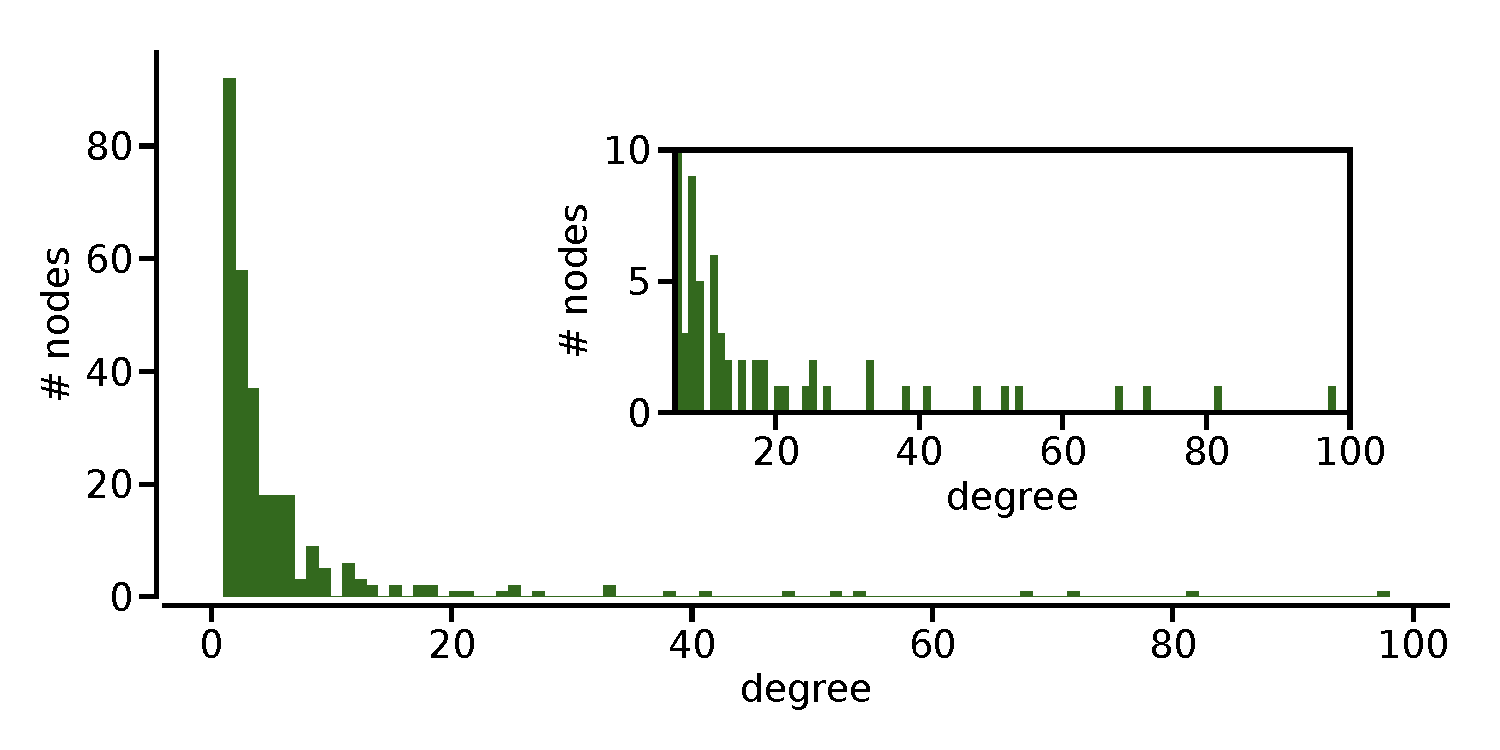
\includegraphics[width=1.0\textwidth]{figures/in-degree_distribution} \\
    (b) In-Degree Distribution
    \end{minipage}
  \end{minipage}
  \caption[In-Degree Distribution of the Citation Network]{\textbf{In-Degree Distribution.} The in-degree distribution describes how often articles get referred by other articles. The long tail of the distribution indicates that there are a lot of articles which are cited only a few times, and a few articles which are cited more often. There are some outliers with a higher degree than $20$. This can also be seen by the difference between the mean and the median. The maximum number of references in connection with the zoomed view represents that one single article was cited by $98$ other articles.}
  \label{fig:indegree_distribution}
\end{figure}

\Cref{fig:indegree_distribution} describes the in-degree distribution of our citation network. In general, the in-degree of a node is the number of ingoing edges. The in-degree distribution represents the probability distribution of these nodes over the whole network. Regarding a citation network the in-degree of a node is the number of articles which referred to this article. The long tail of the in-degree distribution indicates that there are a lot of articles which are referred only a few times, and a few articles which are referred more often. There are only some articles with an in-degree higher than $20$. The maximum number of references in connection with the zoomed view represents that one single article was referred by $98$ other articles.

\begin{figure}[!t]
  \begin{minipage}[!t]{\textwidth}
    \begin{minipage}[b]{0.39\textwidth}
      \centering
      \begin{tabular}{ l c }
        \toprule
        \textbf{Max References}    & $13$     \\ \midrule
        \textbf{Mean References}   & $2.4034$ \\ \midrule
        \textbf{Median References} & $2$      \\
        \bottomrule
    \end{tabular} \\
    \vspace*{1cm}
    (a) Properties
  \end{minipage}
  \begin{minipage}[b]{0.59\textwidth}
    \centering
    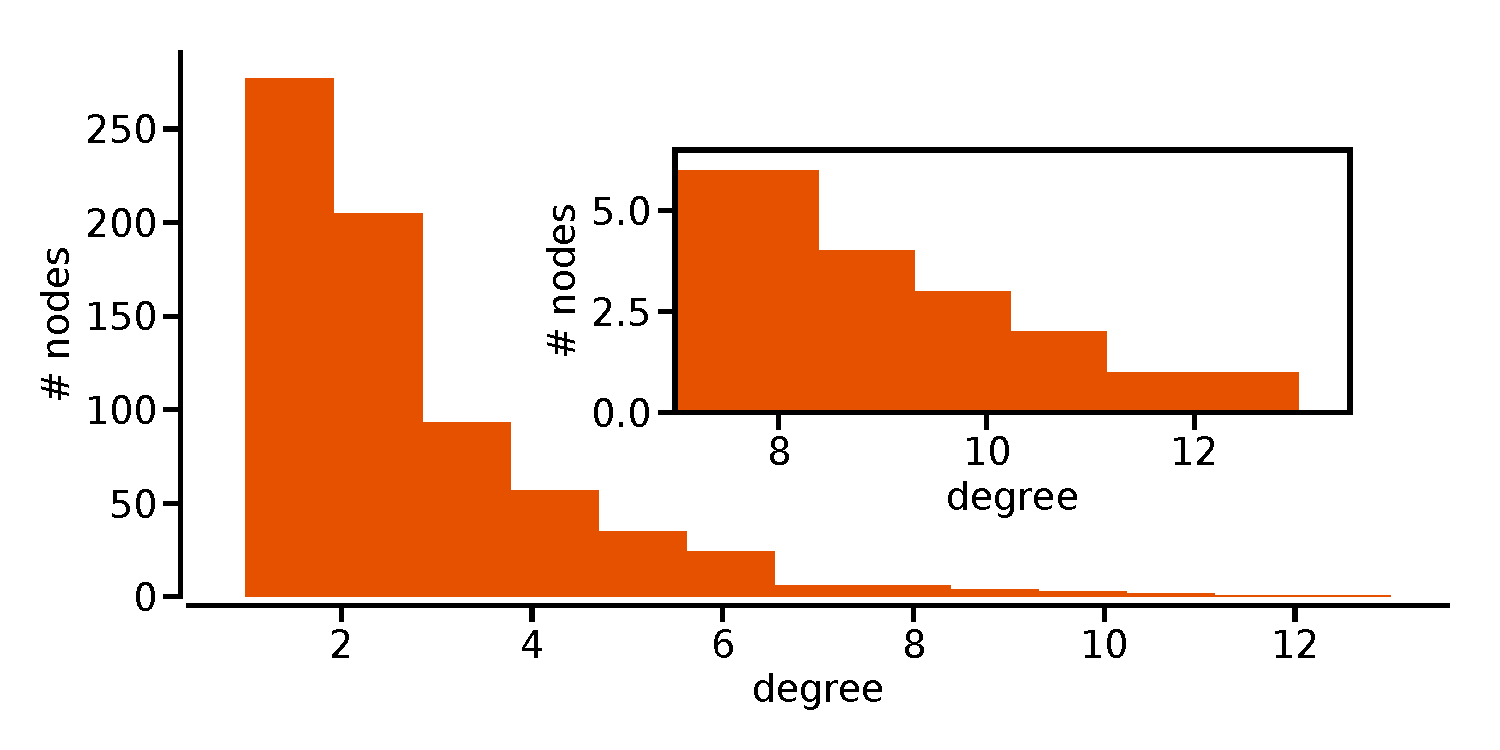
\includegraphics[width=1.0\textwidth]{figures/out-degree_distribution} \\
    (b) Out-Degree Distribution
    \end{minipage}
  \end{minipage}
\caption[Out-Degree Distribution of the Citation Network]{\textbf{Out-Degree Distribution.} The out-degree distribution describes how often articles refer other articles. The long tail of the distribution indicates that there are a lot of articles which refer less than $7$ other articles, and only few with refer to more articles. Mean and median of the outgoing edges are low, because not every refereed article is part of our dataset. By the small difference between the mean and the median can be seen that there are less outliers. The maximum number of references represent that the highest number of a single article refers other articles is $13$.}
\label{fig:outdegree_distribution}
\end{figure}

The out-degree distribution and their properties are displayed in \Cref{fig:outdegree_distribution}. In contrast to the in-degree distribution, the out-degree distribution describes the number of outgoing edges. Regarding to the citation network, the out-degree of a node can be described as the number of articles which gets referred by this article. The long tail of the out-degree distribution indicates that there are a lot of articles which refer less than $7$ other articles, and only few with refer $7$ or more articles. Mean and median of the outgoing edges are low, because not every refereed article is part of our dataset. By the small difference between mean and median we can also see that there are less outliers. The maximum number of references represent the highest number of a single article refers to other articles, which is in our case $13$.

\section{Model}
\label{sec:model}

An information retrieval model is defined by the quadruple $[\textbf{D}, \textbf{Q}, \mathcal{F}, \mathcal{R}(q_i, d_j)]$ that contains the design of documents in the document collection, queries, the framework, and the ranking function (cf. \Cref{sec:information_retrieval_models}). We designed our system to compare various common ranking algorithms. Therefore we generated a model where ranking algorithm can easily be changed by a config parameter.

The document definition was one of the most challenging parts, as our evaluated ranking algorithms need various data sources. Furthermore, 



%\subsection{Query Structure}

%Write how a query looks like - explicit and implicit

%\subsection{Introducing IMRaD Structure Features into Weighing Schemes}

%Write how the algorithms described in \Cref{sec:unstructured_text_Retrieval} are modified for IMRaD structure features.
